\documentclass[12pt]{article}
\setlength{\oddsidemargin}{0in}
\setlength{\evensidemargin}{0in}
\setlength{\textwidth}{6.5in}
\setlength{\parindent}{0in}
\setlength{\parskip}{\baselineskip}

\usepackage{amsmath,amsfonts,amssymb,graphicx,enumerate,float}

\begin{document}

CSCI 5454 \hfill Problem Set 4\\
Robert Werthman\\
No Collaborators

\hrulefill

\begin{enumerate}
  \item \textit{Implement the action setting of Hedge and use it to complete a
  few tasks.}
  	\begin{enumerate}
  	  \item \textit{Use Hedge to write a game AI and display some sample output.}
  	    \scriptsize
  	  	\begin{verbatim}
	 	Payoff Matrix
		[-8, 10, 2]
		[-4, -2, -1]
		[-8, -6, 1]
		##########
		Round 0
		##########
		Enter the row you wish to choose: 0
		Action chosen by user 0
		Probability distribution of AI actions [0.3333333333333333,0.3333333333333333,0.3333333333333333]
		Action chosen by AI 1
		AI loss vector [-8, 10, 2]
		AI weight vector [2980.9579870417283, 4.5399929762484854e-05, 0.1353352832366127]
		old AI score 0.0 , new AI score -10.0 , difference -10.0
		old user score 0.0 , new user score 10.0 , difference 10.0
		##########
		Round 1
		##########
		Enter the row you wish to choose: 0
		Action chosen by user 0
		Probability distribution of AI actions [0.9999545869027009, 
		1.522928810416062e-08, 4.5397868011057175e-05]
		Action chosen by AI 0
		AI loss vector [-8, 10, 2]
		AI weight vector [8886110.520507872, 2.061153622438558e-09, 0.018315638888734182]
		old AI score -10.0 , new AI score -2.0 , difference 8.0
		old user score 10.0 , new user score 2.0 , difference -8.0
		##########
		Round 2
		##########
		Enter the row you wish to choose: 0
		Action chosen by user 0
		Probability distribution of AI actions [0.9999999979388461,2.319522825462676e-16,2.0611536181902033e-09]
		Action chosen by AI 0
		AI loss vector [-8, 10, 2]
		AI weight vector [26489122129.84347, 9.357622968840175e-14, 0.002478752176666359]
		old AI score -2.0 , new AI score 6.0 , difference 8.0
		old user score 2.0 , new user score -6.0 , difference -8.0
  		\end{verbatim}
  	  	\normalsize
  	  \item \textit{Give a plot that exhibits $\Theta{(\sqrt{T})}$ regret.}
  	    \begin{figure}[H]
  	    \centering
  	    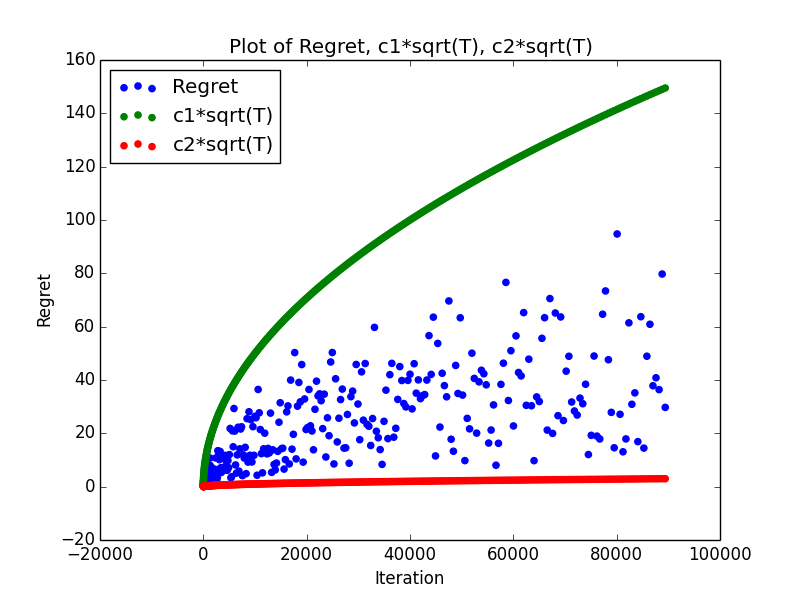
\includegraphics[width=9cm]{q1b.png}
  	    \end{figure}
  	    I let $c_1 = .5$ and $c_2 = .01$ and $\eta = \sqrt{\frac{8ln\,N}{T}}$. 
  	    The graph shows that regret is bounded by $\Theta{(\sqrt{T})}$ where T is the number of rounds. Regret remained
  	    $\le \sqrt(\frac{T}{2}ln\,N)$.  At times regret would get really close to
  	    the bound but other times it would not be close.  It never went above the
  	    bound. Example output of regret in the first column and
  	    $\sqrt(\frac{T}{2}ln\,N)$ in the second column is below.
  	    \scriptsize
  	    \begin{verbatim}
		0.0854754326956 1.16388787282
		0.711207959794 1.55185049709
		0.915738476176 1.93981312136
		1.86659059913 2.32777574563
		1.11868740447 2.7157383699
		0.942107984927 3.10370099418
		1.20108924348 3.49166361845
		2.33209799223 3.87962624272
		2.39799236386 4.26758886699
		3.71141140061 4.65555149126
		3.10138106514 5.04351411554
		1.19507429131 5.43147673981
		3.95892727292 5.81943936408
		0.926603427611 6.20740198835
		2.69832933191 6.59536461262
		0.594289924894 6.9833272369
		6.25916816147 7.37128986117
		3.62512254793 7.75925248544
		0.855690231446 8.14721510971
  	    \end{verbatim}
  	    \normalsize
  	\end{enumerate}
  	
  \newpage
  \item \textit{Show that squared loss guarantees that the best prediction
  in terms of expected loss is going to be x = p.  Give a distribution where
  this is not the case for absolute loss.}\\
  \\
  We want to prove that the expected loss $E[L(x,y)]$ is minimized by letting
  $x=p$.  If $y = 1$ with probability $p$ and $y = 0$ with probability $1-p$
  then 
  \begin{align*}
  E[L(x,y)] &= p \cdot L(x,1) + (1-p) \cdot L(x,0)\\
  &= p \cdot (x-1)^2 + (1-p) \cdot x^2\\
  &= p \cdot (x^2 - 2x + 1) + (1-p)\cdot x^2\\
  &= px^2 - 2px + p + x^2 - px^2\\
  & = x^2 - 2px + p\\
  \end{align*}
  The minimum of a quadratic function of the form $f(x) = ax^2 + bx +c$ can be
  found with the equation 
  $$
  x = -\frac{b}{2a}
  $$
  Solving for $x$ we get 
  $$
  -1 \cdot \frac{(-2px)}{2 \cdot 1} = \frac{2p}{2} = p
  $$
  This shows that the minimum expected loss occurs when is $x=p$.\\
  \\
  Now we want to show that there is a probability distribution for $y=1$ and
  $y=0$ where the expected value of the absolute loss function is not minimized
  when $x=p$.  We can write the expected value of the absolute loss function
  when $y=1,0$ as $$
  E[L(x,y=1,0)] = z|x-1| + w|x-0|
  $$
  where $z$ is the probability of $y=1$ and $w$ is the probability of $y=0$. 
  Since we can assume $x \ge 0$ we can write the expected value of the
  absolute loss function above as
  \begin{align*}
  E[L(x,y=1,0)] &= z(x-1) + wx\\
  \end{align*}
  If we let $z=p$ and $w=1-p$ then the expected value of the absolute
  loss function is
  \begin{align}
  (p)(x-1) + (1-p)x = px - p + x -px = -p + x 
  \end{align}
  
  I have no solution for this part of the problem.
  
  \newpage
  \item \textit{Use hedge as a subroutine and give an algorithm with will
  always achieve $O(\sqrt{T})$ regret without knowing T ahead of time.}\\
  \\
  \textbf{Pseudocode}\\
  \begin{verbatim}
  def MetaHedge():
    set learning rate to the 1/sqrt(time_horizon_guess).
    start Hedge with inputs time_horizon_guess and learning_rate.
    update the learning rate with a new time_horizon_guess everytime 
    the rounds (T) of the learning algorithm exceed time_horizon_guess. 
  \end{verbatim}
  \textbf{Correctness}\\
  \\
  The solution to this question is using the time horizon guess $\hat{T}$ change
  the learning rate $\eta$ as the algorithm runs in order to keep the regret $O(\sqrt{T})$.  Two cases arise
  with this algorithm when we don't know how many rounds it will run for.
  \begin{enumerate}
    \item The algorithm stops before or at the time horizon guess
    $\hat{T}$.  In this case $\hat{T}$ will be $\ge T$, where $T$ is the
    actual number of rounds the algorithm ran for.  Since we overestimate or
    extimate exactly $T$ with $\hat{T}$, the learning rate $\eta$ and the
    weights and the losses will be as expected or smaller then expected. 
    Because of this when we sum the algorithm loss and the minimum loss of the
    single best predition/action to get regret it will be bounded by
    $O(\sqrt{T})$.
    \item The number of rounds $T$ the algorithm runs for exceeds the time
    horizon guess $\hat{T}$.  An example of this is if we set $\hat{T} = 3$ but
    $T$ ends up running for 4 rounds instead.  In this case once $T=3$ we would
    guess $\hat{T} > 3$ taking us back to the first case above.  We would do
    this over and over again until the algorithm stopped.
  \end{enumerate}
  In both of these cases the regret remains below $\sqrt{T}$ because we
  overestimate the number of rounds $T$ the algorithm runs for with
  time horizon guess $\hat{T}$ which gives us a smaller learning rate $eta$ and
  consistently smaller loss and weight vectors.
  \newpage
  \item \textit{Design an online selling algorithm which will maximize the
  number of customers helped in a hardward store with limited supplies.}
    \begin{enumerate}
      \item
      \item
      \item
    \end{enumerate}
    
  \newpage
  \item \textit{Find a mixed nash equilibrium of the zero-sum game.  Give both
  strategies and the value of the game and show the vector of expected payoffs
  for player 2 under player 1's strategy and vice versa.}
    $$
    M = \begin{bmatrix}
        1 & 0 & 1 & 8 & 0\\
        5 & 8 & 9 & 2 & 1\\
        0 & 1 & 8 & 0 & 5\\
        8 & 9 & 2 & 1 & 0\\
        1 & 8 & 0 & 5 & 8\\
        \end{bmatrix}
    $$
  Nash equilibrium means that player 1 and player 2 won't want to deviate from
  their strategies.  The row player wants to minimize and the column player
  wants to maximize.
    
\end{enumerate}


\end{document}